\chapter{A-priori wall-function assessments}
\label{app:zpg:apriori}

This appendix supplements Section~\ref{sec:comparative:zpg:cross-comparison}
with Li and Griffin assessments for the additional Zhang cases M2p5,
M6Tw076, M8Tw048 and M14Tw018. The prescribed-profile procedure is unchanged.
For adiabatic M2p5, relative heat-flux errors are undefined. The M6Tw076
heat-flux curves are retained for completeness, subject to the reference-data
limitations in Section~\ref{sec:evaluation:benchmark-cases}.

\section{Zhang cases}

% Figure provenance and reproducible replot for all eight assessments:
%   Script: 07_Error_Isolation_Results/Figures/Closures/plot_apriori_assessments.py
%   Exact saved solver sweeps, original WSL paths and SHA256 hashes:
%     07_Error_Isolation_Results/Figures/Closures/apriori_sources/manifest.json
%   Shear is shown left and heat flux right. The original 10.5 pt plotting
%   font and 0.85-linewidth inclusion are retained; each case occupies one page.

\begin{figure}[H]
    \centering
    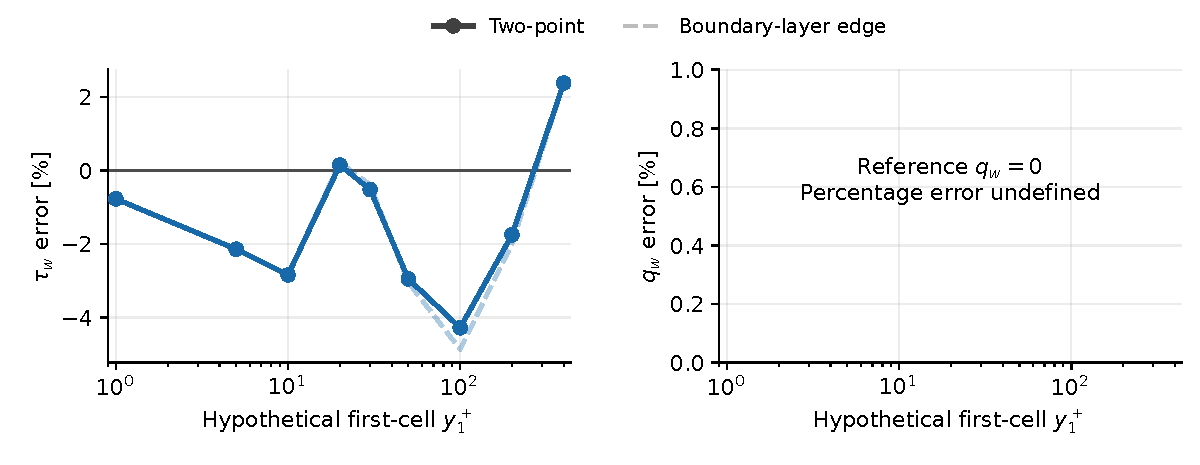
\includegraphics[width=0.85\linewidth]{07_Error_Isolation_Results/Figures/Appendix/a-priori/02_a-priori_Li_M2p5.pdf}
    \caption[M2p5: a-priori Li wall-function assessment]{A-priori Li assessment for M2p5; \(Re_\tau = 510\) \cite{zhang2018direct}. Signed relative errors in wall shear stress \(\tau_w\) (left) and heat-flux \(q_w\) (right) versus \(y_1^+\). Solid: equal-height two-cell formulation; dashed: boundary layer-edge reference. The heat-flux percentage error is undefined for this adiabatic reference.}
    \label{fig:app:zpg:apriori:Li-M2p5}
\end{figure}

\begin{figure}[H]
    \centering
    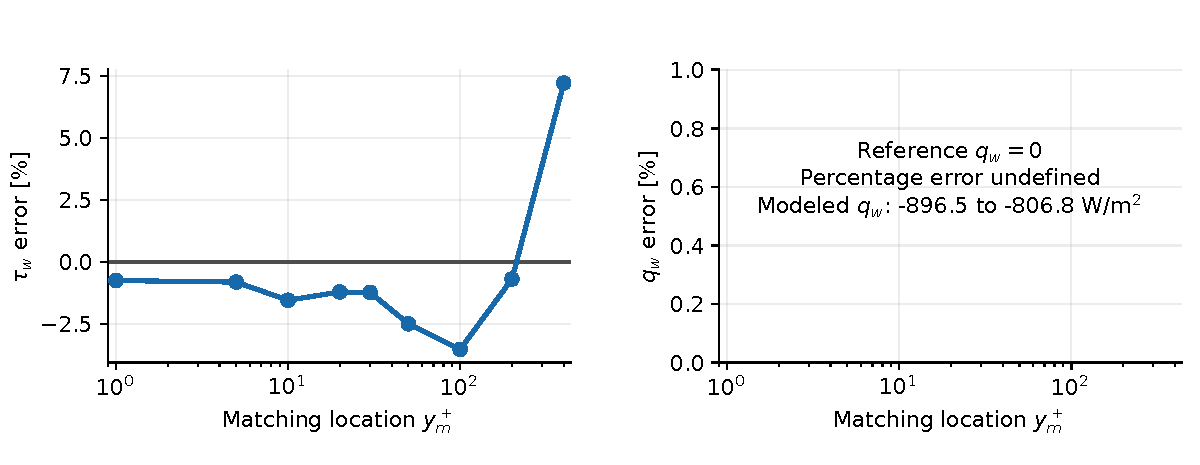
\includegraphics[width=0.85\linewidth]{07_Error_Isolation_Results/Figures/Appendix/a-priori/Griffin_M2p5.pdf}
    \caption[M2p5: a-priori Griffin wall-function assessment]{A-priori assessment of the Griffin wall function for M2p5; \(Re_\tau = 510\) \cite{zhang2018direct}. Signed relative errors in wall shear stress \(\tau_w\) (left) and wall heat-flux \(q_w\) (right) versus matching height \(y_m^+\). The relative heat-flux error is undefined because the reference heat-flux is zero.}
    \label{fig:app:zpg:apriori:Griffin-M2p5}
\end{figure}

\clearpage

\begin{figure}[H]
    \centering
    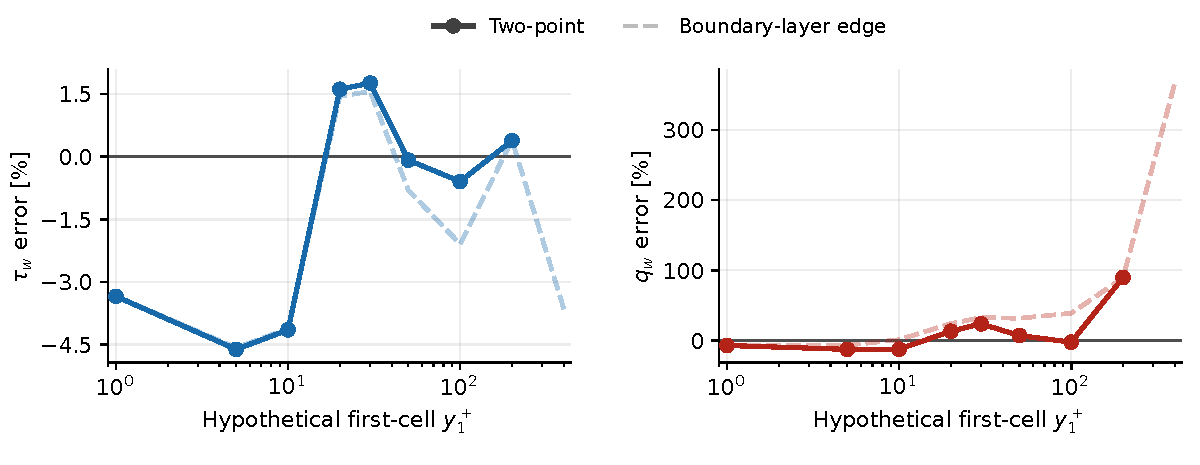
\includegraphics[width=0.85\linewidth]{07_Error_Isolation_Results/Figures/Appendix/a-priori/02_a-priori_Li_M6Tw076.pdf}
    \caption[M6Tw076: a-priori Li wall-function assessment]{A-priori assessment of the Li wall function for M6Tw076; \(Re_\tau = 453\) \cite{zhang2018direct}. Signed relative errors in wall shear stress \(\tau_w\) (left) and wall heat-flux \(q_w\) (right) versus virtual first-cell height \(y_1^+\). Solid curves use the equal-height two-cell formulation; dashed curves use the boundary layer-edge reference. The heat-flux curves are shown for completeness and excluded from quantitative assessment against DNS.}
    \label{fig:app:zpg:apriori:Li-M6Tw076}
\end{figure}

\begin{figure}[H]
    \centering
    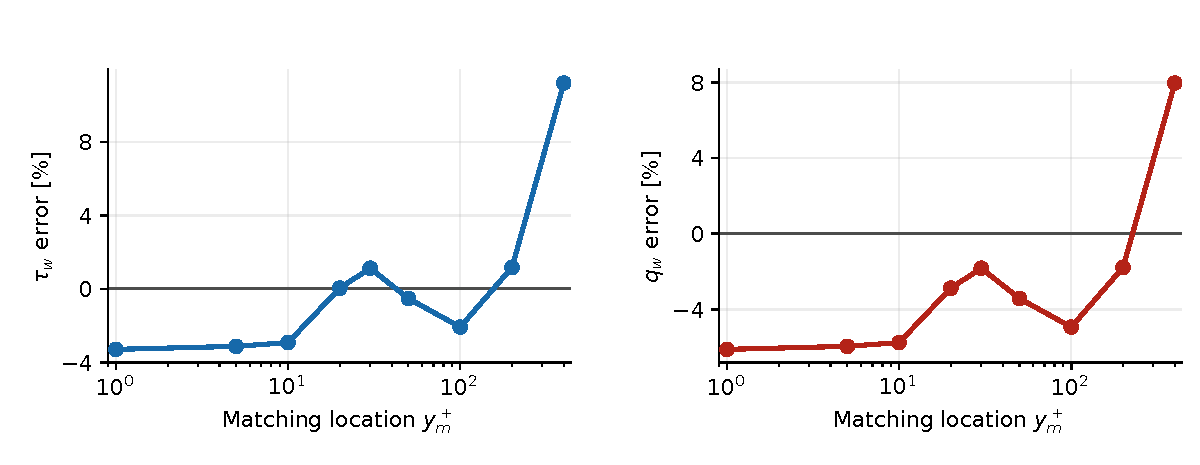
\includegraphics[width=0.85\linewidth]{07_Error_Isolation_Results/Figures/Appendix/a-priori/Griffin_M6Tw076.pdf}
    \caption[M6Tw076: a-priori Griffin wall-function assessment]{A-priori assessment of the Griffin wall function for M6Tw076; \(Re_\tau = 453\) \cite{zhang2018direct}. Signed relative errors in wall shear stress \(\tau_w\) (left) and wall heat-flux \(q_w\) (right) versus matching height \(y_m^+\). The heat-flux curves are shown for completeness and excluded from quantitative assessment against DNS.}
    \label{fig:app:zpg:apriori:Griffin-M6Tw076}
\end{figure}

\clearpage

\begin{figure}[H]
    \centering
    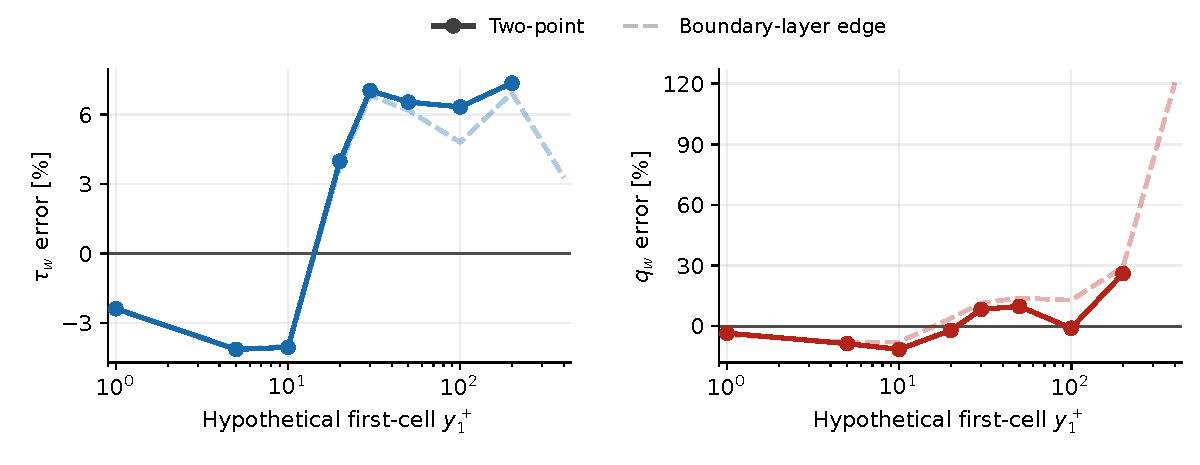
\includegraphics[width=0.85\linewidth]{07_Error_Isolation_Results/Figures/Appendix/a-priori/02_a-priori_Li_M8Tw048.pdf}
    \caption[M8Tw048: a-priori Li wall-function assessment]{A-priori assessment of the Li wall function for M8Tw048; \(Re_\tau = 480\) \cite{zhang2018direct}. Signed relative errors in wall shear stress \(\tau_w\) (left) and wall heat-flux \(q_w\) (right) versus virtual first-cell height \(y_1^+\). Solid curves use the equal-height two-cell formulation; dashed curves use the boundary layer-edge reference.}
    \label{fig:app:zpg:apriori:Li-M8Tw048}
\end{figure}

\begin{figure}[H]
    \centering
    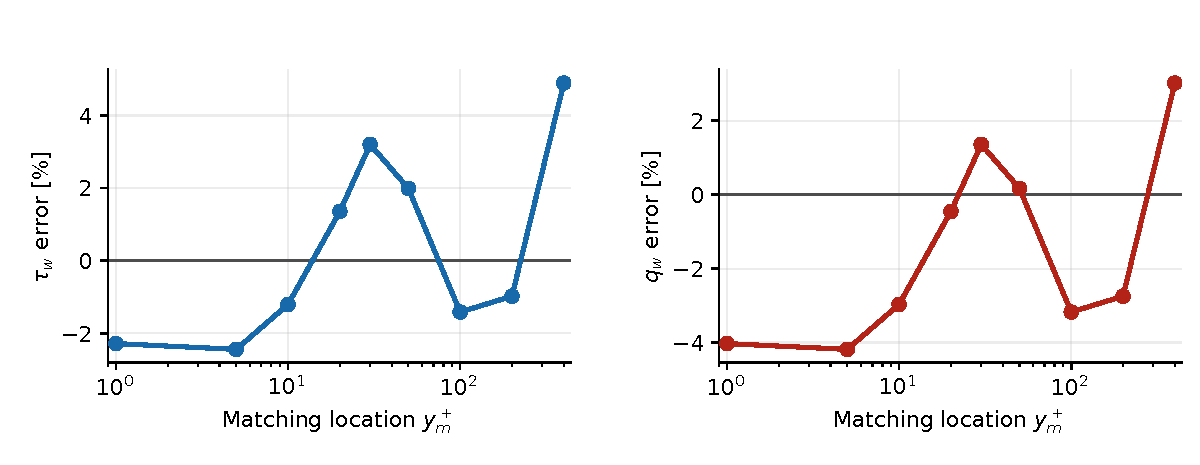
\includegraphics[width=0.85\linewidth]{07_Error_Isolation_Results/Figures/Appendix/a-priori/Griffin_M8Tw048.pdf}
    \caption[M8Tw048: a-priori Griffin wall-function assessment]{A-priori assessment of the Griffin wall function for M8Tw048; \(Re_\tau = 480\) \cite{zhang2018direct}. Signed relative errors in wall shear stress \(\tau_w\) (left) and wall heat-flux \(q_w\) (right) versus matching height \(y_m^+\).}
    \label{fig:app:zpg:apriori:Griffin-M8Tw048}
\end{figure}

\clearpage

\begin{figure}[H]
    \centering
    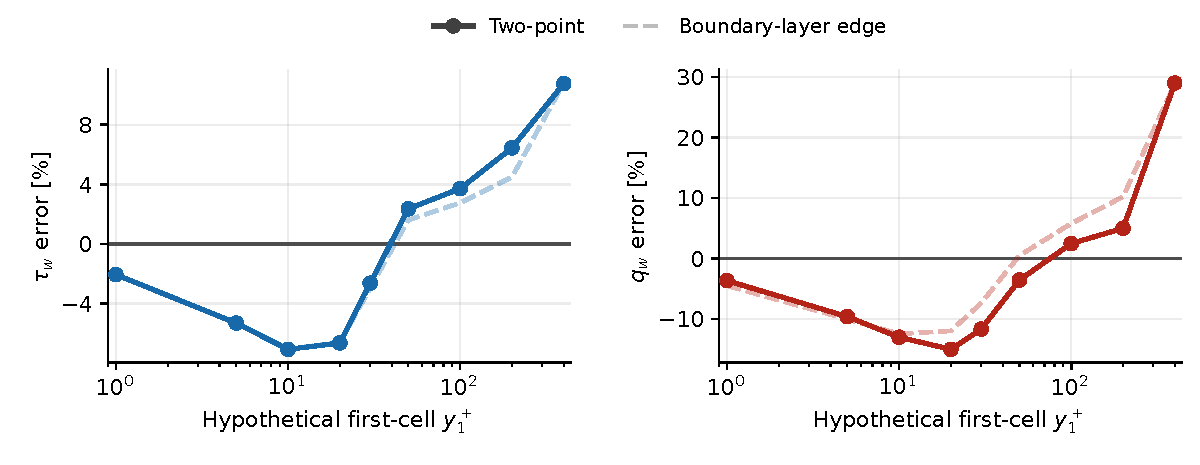
\includegraphics[width=0.85\linewidth]{07_Error_Isolation_Results/Figures/Appendix/a-priori/02_a-priori_Li_M14Tw018.pdf}
    \caption[M14Tw018: a-priori Li wall-function assessment]{A-priori assessment of the Li wall function for M14Tw018; \(Re_\tau = 646\) \cite{zhang2018direct}. Signed relative errors in wall shear stress \(\tau_w\) (left) and wall heat-flux \(q_w\) (right) versus virtual first-cell height \(y_1^+\). Solid curves use the equal-height two-cell formulation; dashed curves use the boundary layer-edge reference.}
    \label{fig:app:zpg:apriori:Li-M14Tw018}
\end{figure}

\begin{figure}[H]
    \centering
    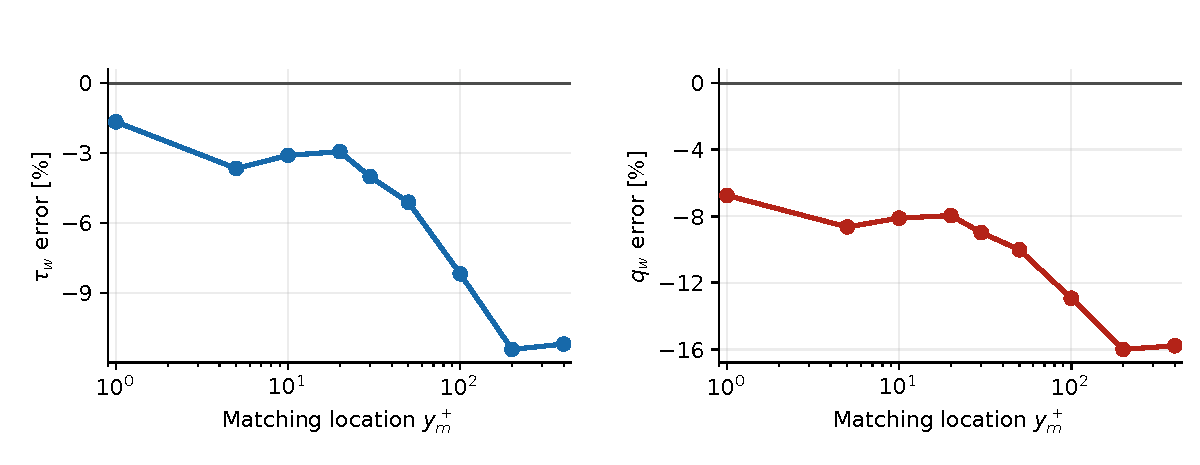
\includegraphics[width=0.85\linewidth]{07_Error_Isolation_Results/Figures/Appendix/a-priori/Griffin_M14Tw018.pdf}
    \caption[M14Tw018: a-priori Griffin wall-function assessment]{A-priori assessment of the Griffin wall function for M14Tw018; \(Re_\tau = 646\) \cite{zhang2018direct}. Signed relative errors in wall shear stress \(\tau_w\) (left) and wall heat-flux \(q_w\) (right) versus matching height \(y_m^+\).}
    \label{fig:app:zpg:apriori:Griffin-M14Tw018}
\end{figure}
